\documentclass[dvipdfmx,autodetect-engine,twocolumn,10pt]{jsarticle}% autodetect-engine で pLaTeX / upLaTeX を自動判定
\setlength{\columnsep}{3zw}
\usepackage[dvipdfmx]{graphicx}
\usepackage{amsmath,amssymb}

\newif\iffigure
\figurefalse
\figuretrue

\title{モンテカルロ法による光子輸送シミュレーションと\\
3次元画像のモンテカルロシミュレーション}
\author{法政大学理工学部 応用情報工学科 4年 16X3128 馬場俊弥}
\date{2019年5月25日}

\begin{document}

\maketitle
\section{はじめに}
SPECT(Single Photon Emission Computed Tomography)とは放射性同位元素(RI:Radio Isotope)を用いた放射性医薬品を体内に投与することによって,放射性医薬品から出る微量な放射線($\gamma$線)を様々な方向から測定し,断層画像にする方法である.

SPECTによる測定において,$\gamma$線を収集する方向を一定にするために,コリメータと呼ばれる装置を用いる.コリメータにはシングルピンホールコリメータ,マルチピンホールコリメータ,パラレルホールコリメータなどがある.コリメータのピンホールは本来円形をしているが,ピンホールの形が矩形である,矩形マルチ矩形ピンホールSPECTの開発を行っている.この研究を進めるにあたり今回は,モンテカルロ法による光子輸送シミュレーション,そして円形のシングルピンホールコリメータを用いた3次元画像のモンテカルロシミュレーションの投影結果を紹介する.

\section{モンテカルロ法による光子輸送シミュレーション}
モンテカルロ法とは,シミュレーションや数値計算を乱数を用いて反復計算を行うことにより,確率的に問題の解を推定する方法である.
1個の光子輸送のフローチャートを図\ref{photon_flow}に示す.
\newpage
\iffigure
  \begin{figure}[htbp]
    \begin{center}
      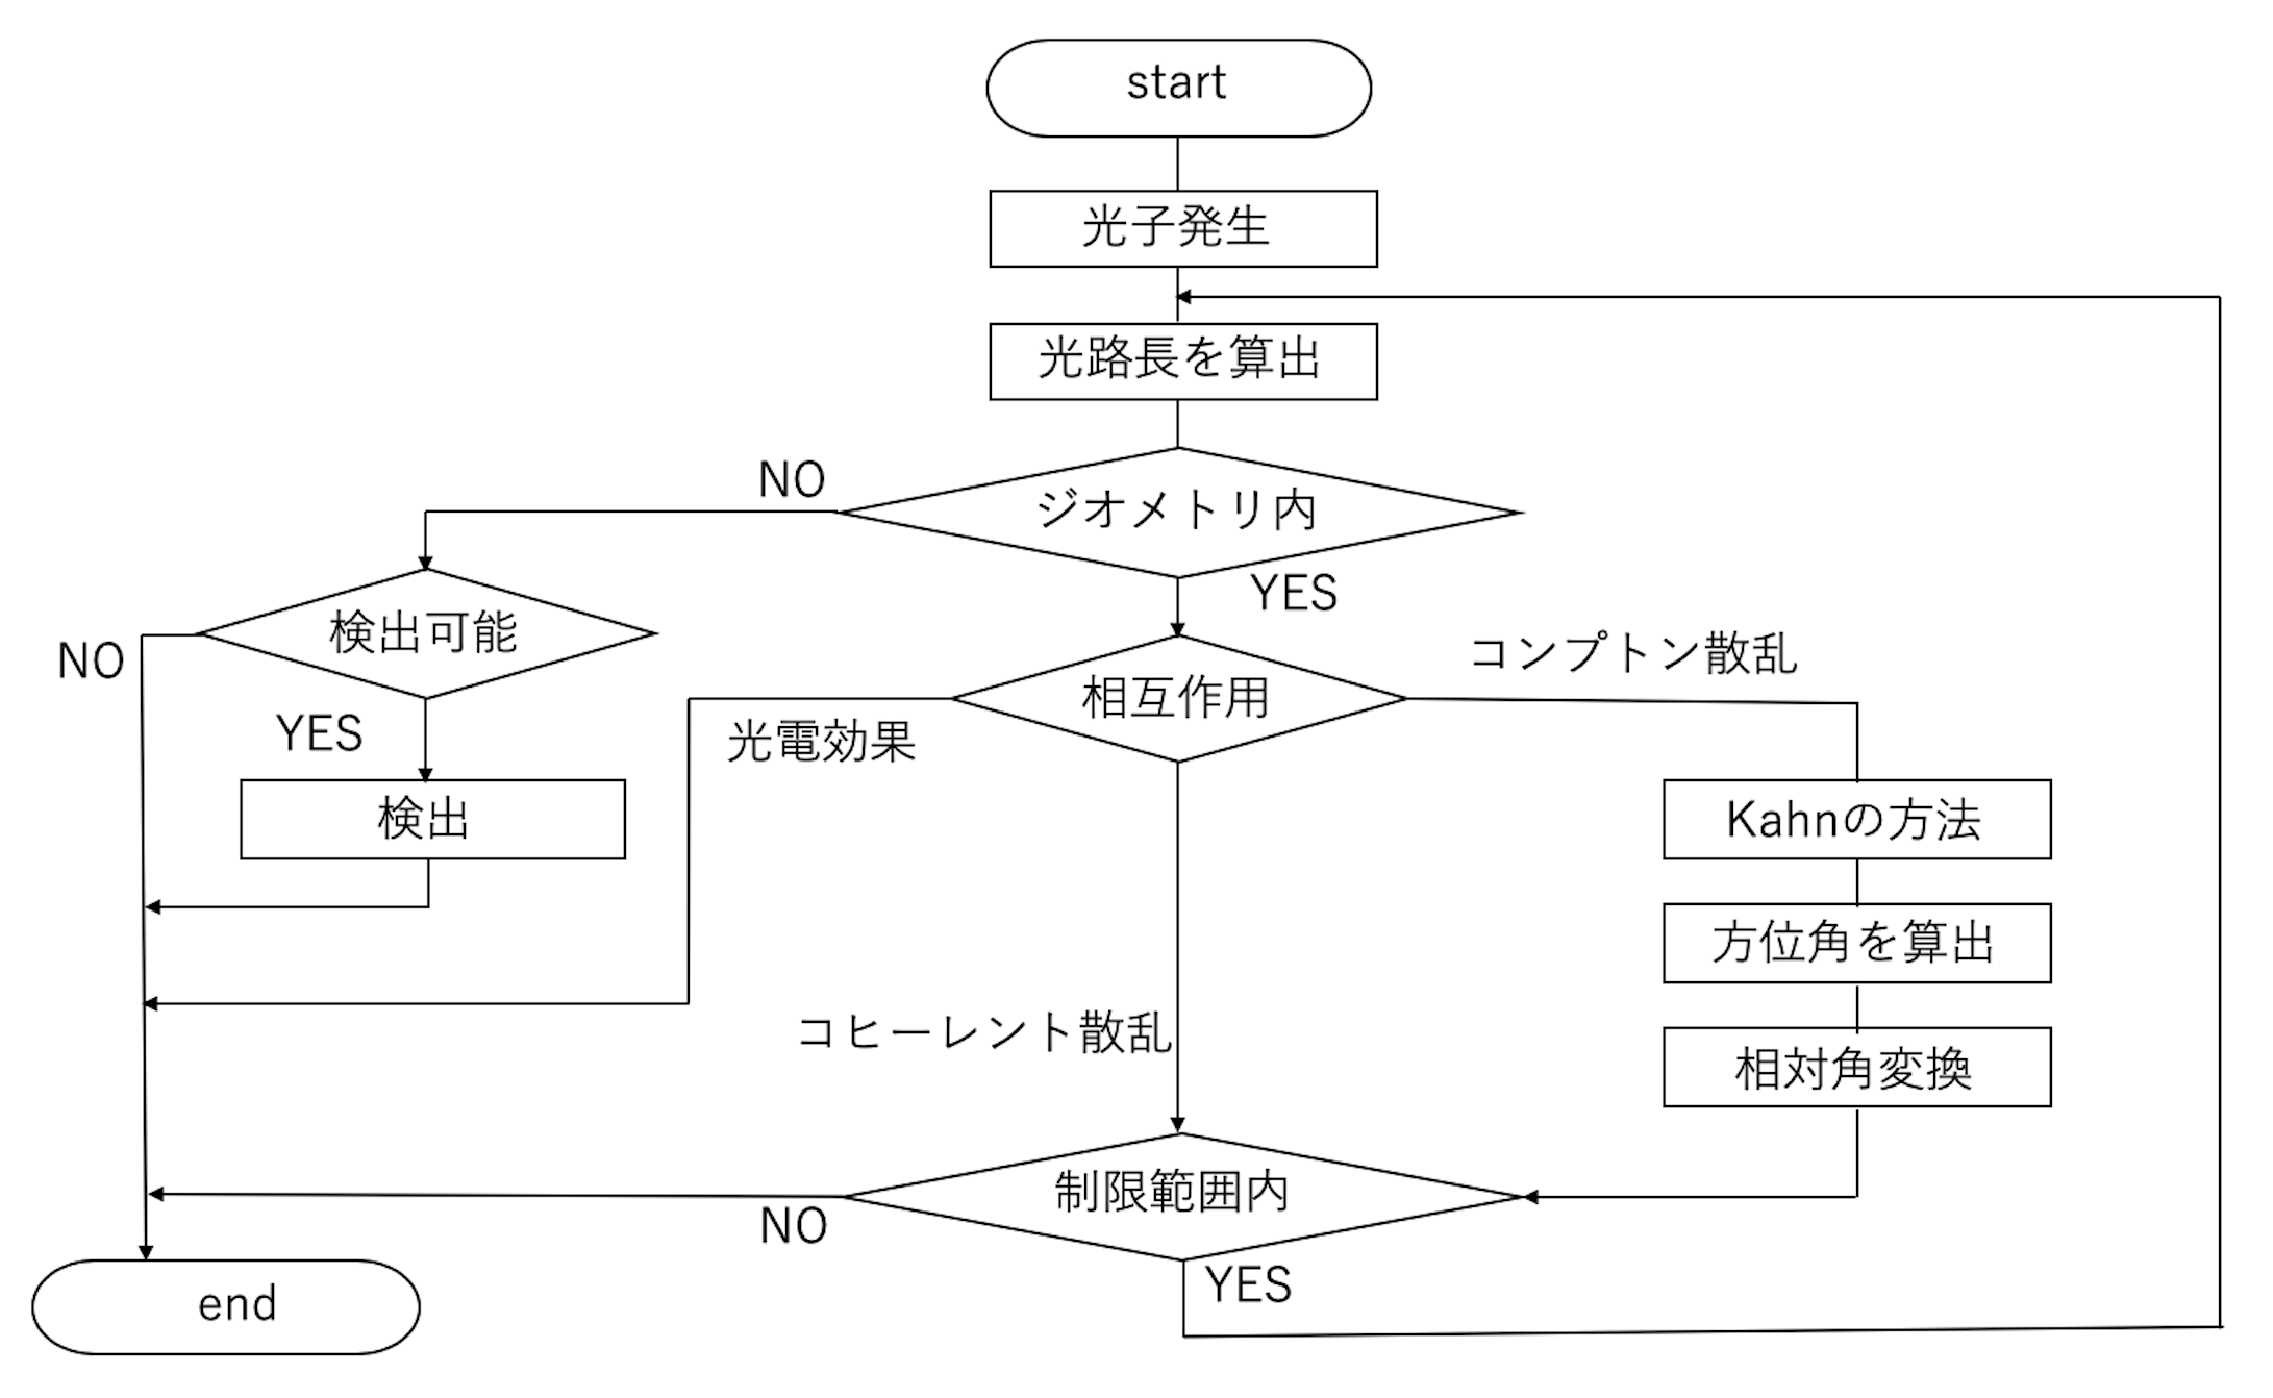
\includegraphics[height=4.4cm]{./file/monte_simu_flow.eps}
      \caption{光子輸送のフローチャート}
      \label{photon_flow}
    \end{center}
  \end{figure}
\fi

図1のように,光子は相互作用を引き起こす.今回のシミュレーションではコンプトン散乱,コヒーレント散乱,光電効果の3つの相互作用を考慮する.コンプトン散乱とは,電子に光子が衝突すると、光子は一部のエネルギーを電子に与え、その分、光子自身はエネルギーが減少し、かつ、進行方向を変えて進むこと,コヒーレント散乱とは,電子と光子が衝突するが、光子のエネルギーはわずかにしか減少せず、光子の進行方向は変わらずに進むこと,光電効果とは電子に光子が衝突すると、光子の全てのエネルギーが電子に吸収されてしまい、その光子は消滅することを意味する.

\section{3次元画像のモンテカルロシミュレーション}
モンテカルロ法による光子輸送シミュレーションを利用して,3次元画像のモンテカルロシミュレーションを行った.矩形ピンホールコリメータとの比較を行うために,まずは円形のピンホールコリメータとの比較を行うために.媒質を水($H_2O$)とした球の画像を使用して投影を行った.

\section{シミュレーション}
\subsection{モンテカルロ法による光子輸送シミュレーション}
モンテカルロ法による光子輸送シミュレーションのシミュレーション条件を表\ref{simu_cond}に示す.
\begin{table}[htbp]
  \begin{center}
    \caption{シミュレーション条件}
    \label{simu_cond}
    \begin{tabular}{|c|c|} \hline
      媒質 & $H_2O$ \\ \hline
      初期エネルギー & 140 $KeV$ \\ \hline
      光子数 & 1億個 \\ \hline
      最大散乱回数 & 5回 \\ \hline
      光子の初期位置 & 原点 \\ \hline
      光子の放出方向 & z軸正方向 \\ \hline
      検出器のサイズ & 65×65 $pixel$ \\ \hline
      カットオフエネルギー & 30 $KeV$ \\ \hline
    \end{tabular}
  \end{center}
\end{table}
\subsection{3次元画像のモンテカルロシミュレーション}
3次元画像のモンテカルロシミュレーションのシミュレーション条件を表\ref{3d_single}に,使用した原画像を図\ref{single_original_img}に示す.
\begin{table}[htbp]
  \begin{center}
    \caption{シミュレーション条件}
    \label{3d_single}
    \begin{tabular}{|c|c|} \hline
      \footnotesize{媒質} & \footnotesize{$H_2O$} \\ \hline
      \footnotesize{発生光子数} & \footnotesize{$50万個/voxel$} \\ \hline
      \footnotesize{初期エネルギー} & \footnotesize{140 $KeV$} \\ \hline
      \footnotesize{最大散乱回数} & \footnotesize{5回} \\ \hline
      \footnotesize{初期散乱角} & \footnotesize{ランダム} \\ \hline
      \footnotesize{初期方位角} & \footnotesize{ランダム} \\ \hline
      \footnotesize{検出器のサイズ} & \footnotesize{512×256 $pixel$} \\ \hline
      \footnotesize{カットオフエネルギー} & \footnotesize{30 $KeV$} \\ \hline
      \footnotesize{原画像サイズ} & \footnotesize{128×128×128 $pixel$} \\ \hline
      \footnotesize{原画像のピクセルサイズ} & \footnotesize{0.2×0.2 $cm^2$} \\ \hline
      \footnotesize{回転半径} & \footnotesize{25 $cm$} \\ \hline
      \footnotesize{コリメータと検出器間の距離} & \footnotesize{7.5 $cm$} \\ \hline
      \footnotesize{ナイフエッジの角度} & \footnotesize{30度} \\ \hline
      \footnotesize{コリメータ径} & \footnotesize{0.5 $cm$} \\ \hline
      \footnotesize{球の半径} & \footnotesize{10 $cm$} \\ \hline
    \end{tabular}
  \end{center}
\end{table}

\iffigure
  \begin{figure}[htbp]
    \begin{center}
      \includegraphics[width=2.5cm]{./file/single_original.png}
      \caption{原画像(128×128×128)}
      \label{single_original_img}
    \end{center}
  \end{figure}
\fi

\newpage
\section{結果}
\subsection{モンテカルロ法による光子輸送シミュレーション}
各散乱回数毎の結果画像とそのプロファイル,エネルギースペクトルをそれぞれ図\ref{monte_result},図\ref{profile},図\ref{energy_spectrum}に示す.
\iffigure

  \begin{figure}[htbp]
    \begin{center}
      \begin{tabular}{c}

        % 1
        \begin{minipage}{0.33\hsize}
          \begin{center}
            
\includegraphics[clip, width=2.4cm]{./file/monte_simu_primary.eps}
            \hspace{1cm} \small{(a)散乱回数0回} \vspace{0.2cm}
          \end{center}
        \end{minipage}

        % 2
        \begin{minipage}{0.33\hsize}
          \begin{center}
            
\includegraphics[clip, width=2.4cm]{./file/monte_simu_1.eps}
            \hspace{1.6cm} \small{(b)散乱回数1回} \vspace{0.2cm}
          \end{center}
        \end{minipage}

        \begin{minipage}{0.33\hsize}
          \begin{center}
            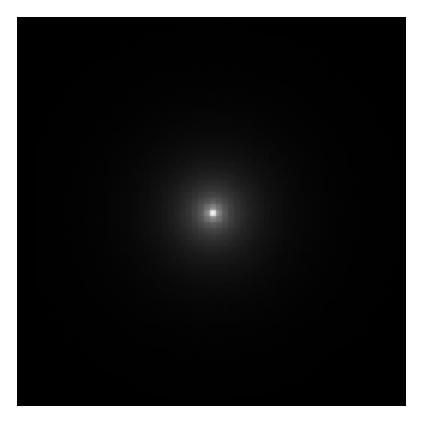
\includegraphics[clip, width=2.4cm]{./file/monte_simu_2.eps}
            \hspace{1.6cm} \small{(c)散乱回数2回} \vspace{0.2cm}
          \end{center}
        \end{minipage}
        \\
        \begin{minipage}{0.33\hsize}
          \begin{center}
            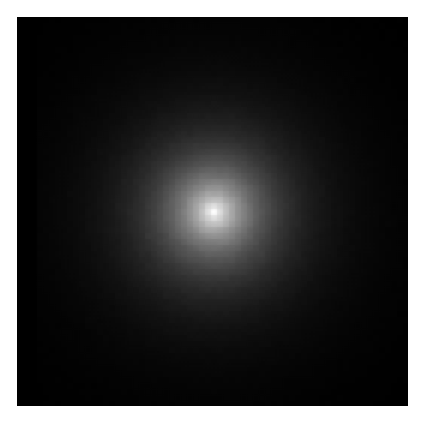
\includegraphics[clip, width=2.4cm]{./file/monte_simu_3.eps}
            \hspace{1.6cm} \small{(d)散乱回数3回} \vspace{0.2cm}
          \end{center}
        \end{minipage}

        \begin{minipage}{0.33\hsize}
          \begin{center}
            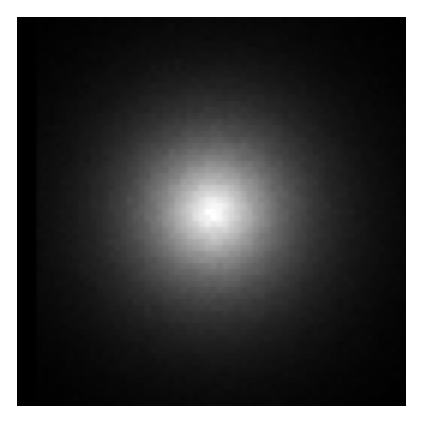
\includegraphics[clip, width=2.4cm]{./file/monte_simu_4.eps}
            \hspace{1.6cm} \small{(e)散乱回数4回} \vspace{0.2cm}
          \end{center}
        \end{minipage}

        \begin{minipage}{0.33\hsize}
          \begin{center}
            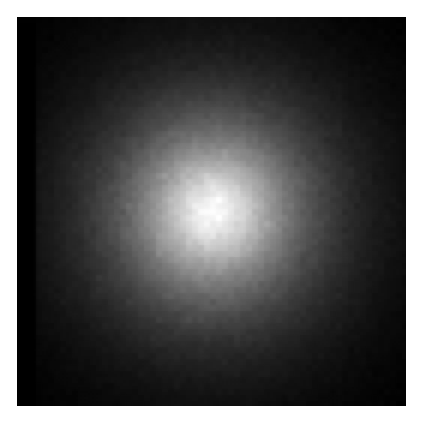
\includegraphics[clip, width=2.4cm]{./file/monte_simu_5.eps}
            \hspace{1.6cm} \small{(f)散乱回数5回} \vspace{0.2cm}
          \end{center}
        \end{minipage}

      \end{tabular}
    \caption{各散乱回数毎の結果画像}
    \label{monte_result}
    \end{center}
  \end{figure}
\fi

\iffigure
  \begin{figure}[htbp]
    \begin{center}
      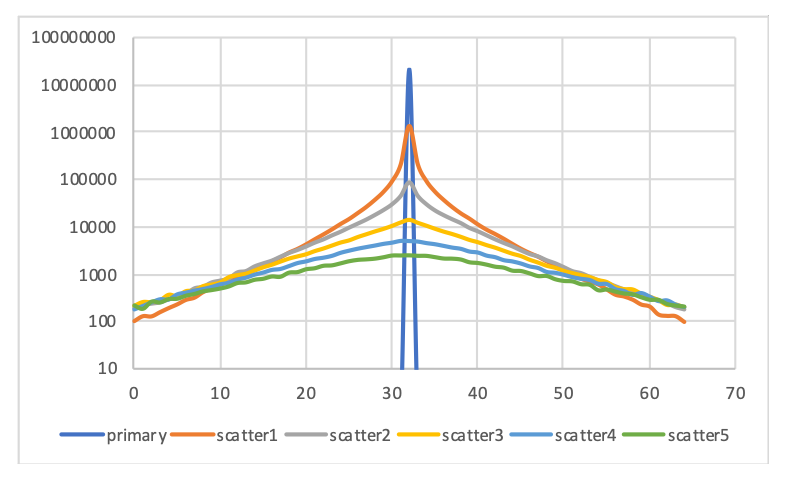
\includegraphics[clip, width=6cm]{./file/monte_profile.eps}
      \caption{プロファイル}
      \label{profile}
    \end{center}
  \end{figure}
\fi

\iffigure
  \begin{figure}[htbp]
    \begin{center}
      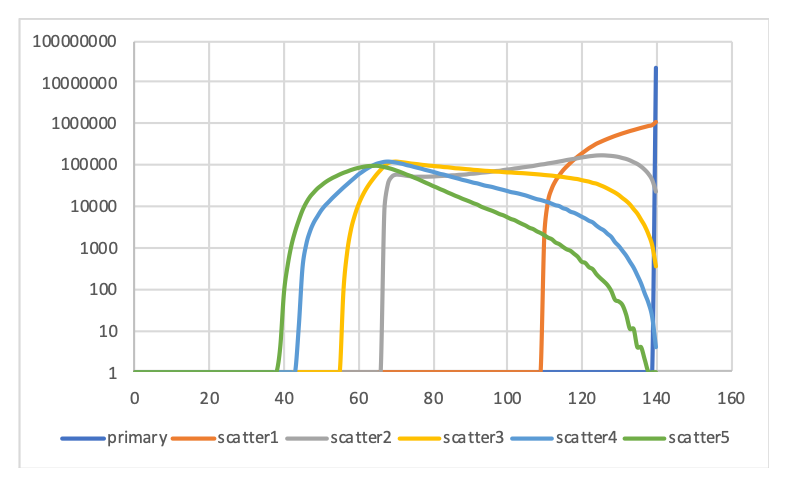
\includegraphics[clip, width=6cm]{./file/monte_energyspec.eps}
      \caption{エネルギースペクトル}
      \label{energy_spectrum}
    \end{center}
  \end{figure}
\fi

\subsection{3次元画像のモンテカルロシミュレーション}
primary光子の投影の結果とそのプロファイルをそれぞれ図\ref{single_proj},\ref{single_proj_profile}に示す.
\iffigure
  \begin{figure}[htbp]
    \begin{center}
      \includegraphics[width=7cm]{./file/primary_float_512-256-180.png}
      \caption{primary光子の投影画像}
      \label{single_proj}
    \end{center}
  \end{figure}
\fi

\iffigure
  \begin{figure}[htbp]
    \begin{center}
      \includegraphics[width=7cm]{./file/single_proj_profile.png}
      \caption{プロファイル}
      \label{single_proj_profile}
    \end{center}
  \end{figure}
\fi

\newpage
\section{まとめと今後の展望}
モンテカルロ法による光子輸送シミュレーションについては理論値との比較を行うことによって正しく実装されていることを確認することができた.今後もこの光子輸送シミュレーションのプログラムを用いて様々なシミュレーションを行っていく.

3次元画像のモンテカルロシミュレーションについては投影は正しく行えていることが確認できたため,有効視野を求めて感度補正,吸収補正を行い,再構成をする.

\end{document}
